% !TeX spellcheck = es_ES
\documentclass[12pt, titlepage]{article}
\usepackage[utf8]{inputenc}
\usepackage[spanish]{babel}
\usepackage{float}
\usepackage[letterpaper, margin=2.5cm]{geometry}
\usepackage[nottoc,notlot,notlof]{tocbibind} % Hace que se agregen las referencias al indice
\usepackage{url}
\usepackage{graphicx} 
\usepackage{listings}
\usepackage{color}
\definecolor{dkgreen}{rgb}{0,0.6,0}
\definecolor{gray}{rgb}{0.5,0.5,0.5}
\definecolor{mauve}{RGB}{253,151,31}

\lstset{frame=tb,
	language=Sql,
	aboveskip=3mm,
	belowskip=3mm,
	showstringspaces=false,
	columns=flexible,
	basicstyle={\small\ttfamily},
	numbers=none,
	numberstyle=\tiny\color{gray},
	keywordstyle=\color{blue},
	commentstyle=\color{dkgreen},
	stringstyle=\color{mauve},
	breaklines=true,
	breakatwhitespace=true,
	tabsize=2,
	morekeywords={use}
}

\title{Reporte: Práctica 8}
\author{Carlos Tonatihu Barrera Pérez \\ Profesor: Hernández Contreras Euler \\ Bases de Datos \\ Grupo: 2CM1 }

\begin{document}
	\maketitle
	\tableofcontents
	\section{Marco Teórico}
	Esperando que este con madre
	\section{Desarrollo}
	En esta práctica se hicieron ejercicios de consultas, altas, cambios y bajas sobre una base con datos sobre un hospital.
	
	El primer ejercicio fue mostrar todos los pacientes.
	\begin{figure}[H]
		\begin{center}
			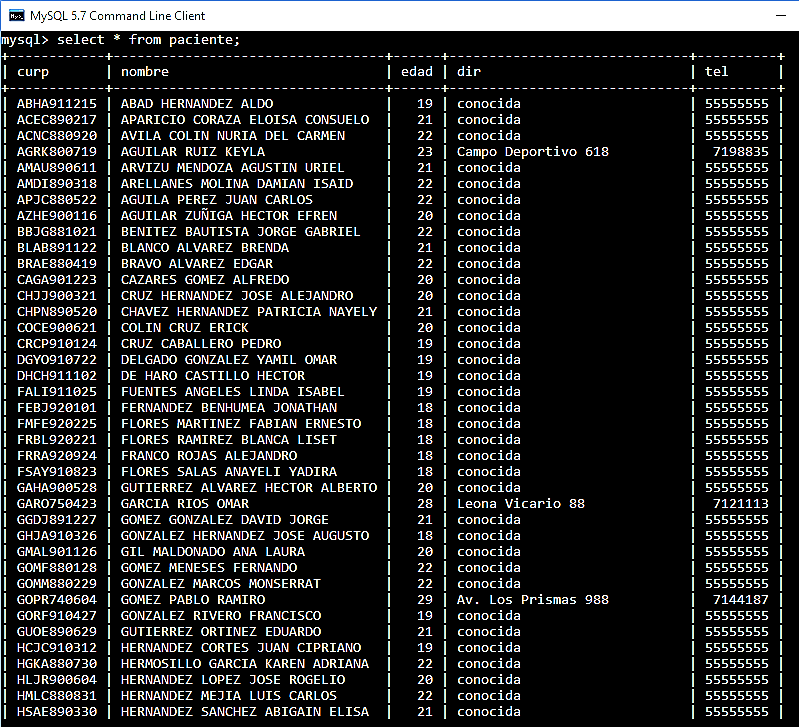
\includegraphics[width=\textwidth]{img/uno.png}
			\label{fig:uno}
			\caption{Todos los pacientes}
		\end{center}
	\end{figure}
	Después se mostró el nombre y edad de dichos pacientes.
	%select nombre, edad from paciente order by 2;%
	\begin{figure}[H]
		\begin{center}
			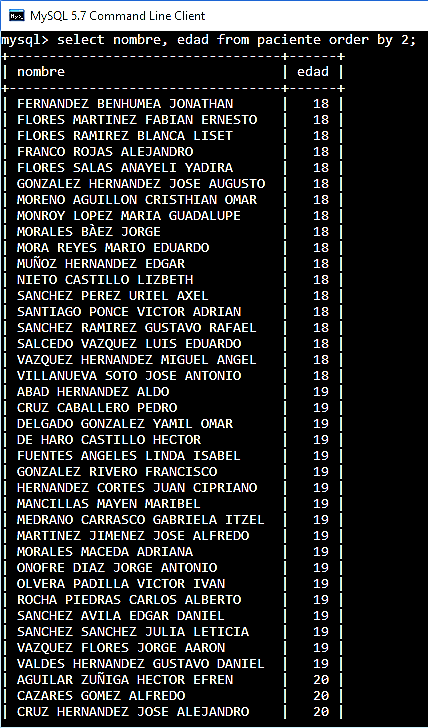
\includegraphics[width=\textwidth]{img/dos.png}
			\label{fig:dos}
			\caption{Datos específicos del paciente}
		\end{center}
	\end{figure}
	A continuación se mostraron los datos del paciente que tiene la siguiente CURP MALD770810
	%select * from paciente where curp like "MALD77%";%
	\begin{figure}[H]
		\begin{center}
			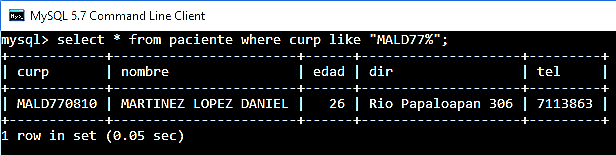
\includegraphics[width=\textwidth]{img/tres.png}
			\caption{Datos del paciente con al CURP solicitada}
			\label{fig:tres}
		\end{center}
	\end{figure}
	Después se mostraron los datos de aquellos pacientes que tienen 26 años, nombre y edad.
	%select nombre, edad from pacientewhere edad=26;%
	\begin{figure}[H]
		\begin{center}
			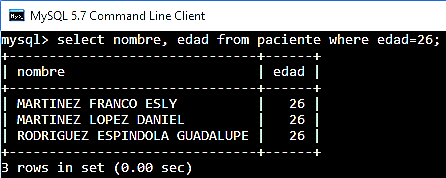
\includegraphics[width=\textwidth]{img/cuatro.png}
			\label{fig:cuatro}
			\caption{Pacientes con 26 años}
		\end{center}
	\end{figure}
	Los siguientes datos fueron los pacientes que tienes más de 25 años de edad.
	%select nombre, edad from paciente where edad>25 order by edad;%
	\begin{figure}[H]
		\begin{center}
			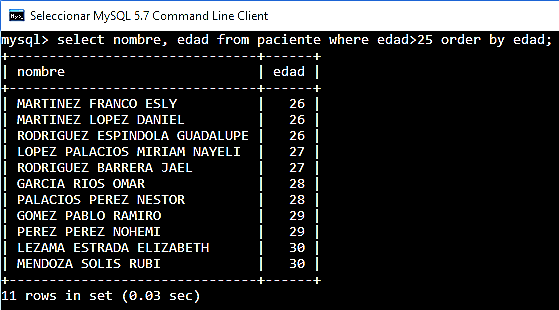
\includegraphics[width=\textwidth]{img/cinco.png}
			\label{fig:cinco}
			\caption{Pacientes que tienen más de 25 años ordenados por edad}
		\end{center}
	\end{figure}
	También se mostró el nombre, y edad de aquellos pacientes cuya edad es igual o mayor a 27 años
	%select nombre, edad from paciente where edad>=27 order by edad;%
	\begin{figure}[H]
		\begin{center}
			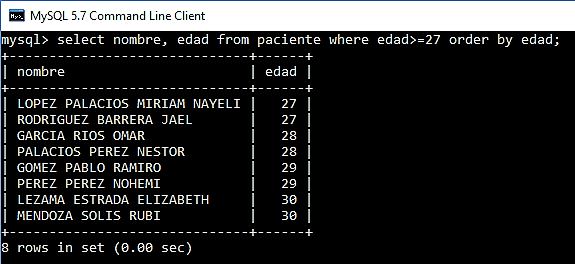
\includegraphics[width=\textwidth]{img/seis.png}
			\label{fig:seis}
			\caption{Datos de pacientes con una edad mayor o igual a 27}
		\end{center}
	\end{figure}
	Lo mismo ocurrió para pacientes que tienen edad menor o igual a 27 años.
	%select nombre, edad from paciente where edad<=27 order by 2;%
	\begin{figure}[H]
		\begin{center}
			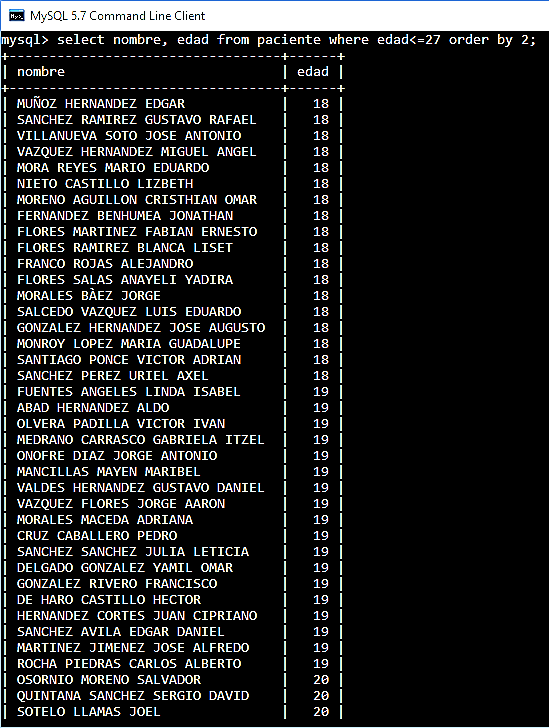
\includegraphics[width=\textwidth]{img/siete.png}
			\label{fig:siete}
			\caption{Lo mismo que la imagen anterior pero con los pacientes menores a 28 años.}
		\end{center}
	\end{figure}
	Luego se mostró el nombre y edad de pacientes que tienen 27 años
	%select nombre, edad from paciente where edad=27 order by 1;%
	\begin{figure}[H]
		\begin{center}
			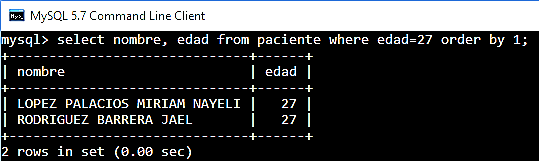
\includegraphics[width=\textwidth]{img/ocho.png}
			\label{fig:ocho}
			\caption{Pacientes con 27 años y sus datos}
		\end{center}
	\end{figure}
	La siguiente consulta fue mostrar los pacientes con 26, 27 y 28 años, para esta consulta se utilizaron las siguientes expresiones.
	\begin{lstlisting}
	select nombre, edad from paciente where edad between 26 and 28 order by 2;
	
	select nombre, edad from paciente where edad in(26,27,28) order by 2;
	
	select nombre, edad from paciente where (edad=26 or edad=27 or edad=28) order by 2;
	\end{lstlisting}
	%Pantallazo%
	\begin{figure}[H]
		\begin{center}
			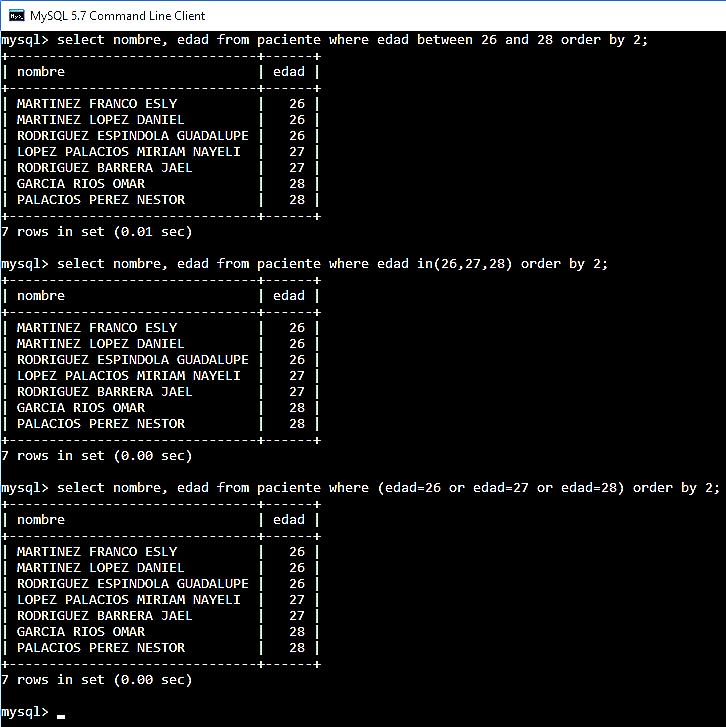
\includegraphics[width=\textwidth]{img/nueve.png}
			\label{fig:nueve}
			\caption{Diferentes formas de mostrar al conjunto de pacientes entre 26 y 27 años}
		\end{center}
	\end{figure}
	
	Para mostrar cuantos pacientes tienen 26 o 28 se utilizo la siguiente instrucción.
	%select nombre, edad from paciente where edad in(26,28) order by 2;%
	\begin{figure}[H]
		\begin{center}
			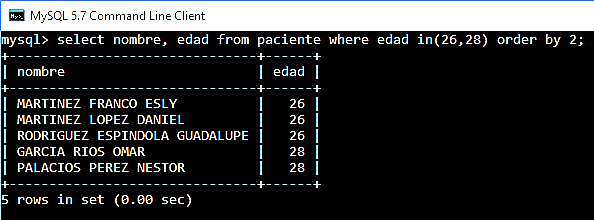
\includegraphics[width=\textwidth]{img/diez.png}
			\label{fig:diez}
			\caption{Pacientes seleccionados}
		\end{center}
	\end{figure}
	
	La siguiente consulta solo muestra a los pacientes de 26 años en adelante pero no a los que tiene 28 años utilizando el signo de diferente en SQL.
	%select nombre, edad from paciente where edad>=26 and edad<>28 order by 2;%
	\begin{figure}[H]
		\begin{center}
			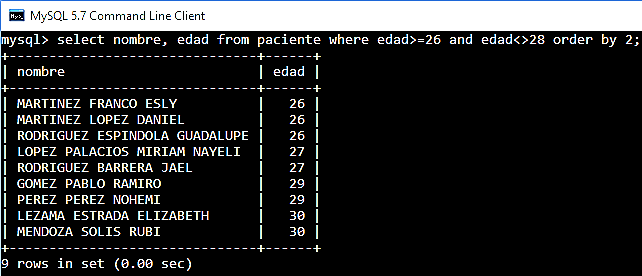
\includegraphics[width=\textwidth]{img/once.png}
			\label{fig:once}
			\caption{No se muestras los pacientes con 28 años a pesar de que se encuentran en el intervalo indicado}
		\end{center}
	\end{figure}
	
	Ahora se muestra el historial de los pacientes que ingresaron el 26 de marzo de 2003.
	%select * from historial where fechaIngreso="2003-03-26";%
	\begin{figure}[H]
		\begin{center}
			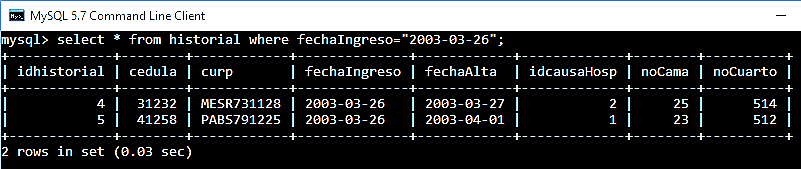
\includegraphics[width=\textwidth]{img/doce.png}
			\label{fig:doce}
			\caption{Pacientes con cierta fecha de ingreso}
		\end{center}
	\end{figure}
	También hacemos lo mismo para los que ingresaron el 25 de ese mismo mes y año.
	%select * from historial where fechaIngreso>"2003-03-25" order by fechaIngreso;%
	\begin{figure}[H]
		\begin{center}
			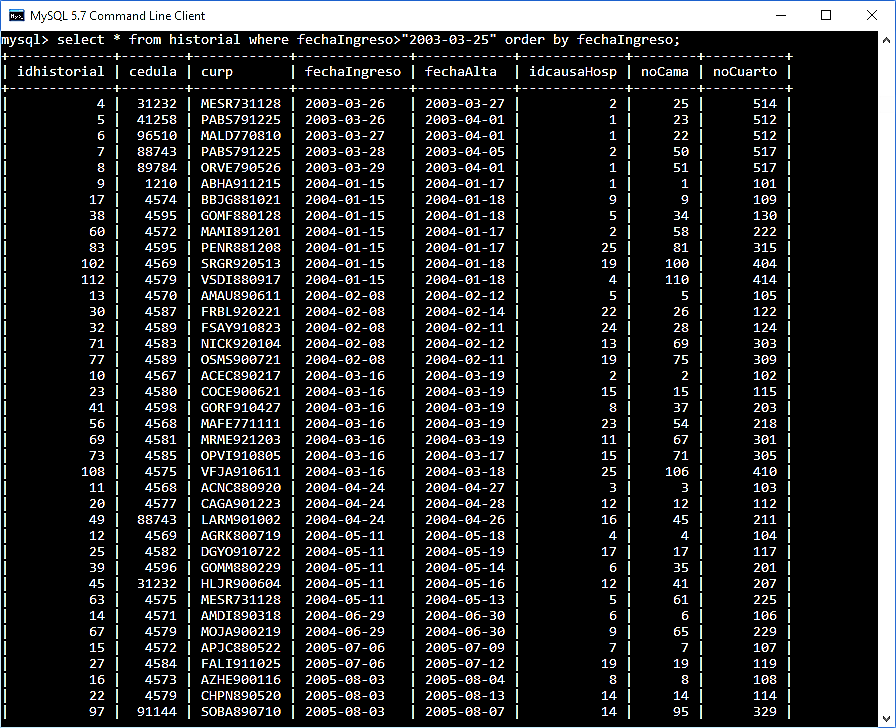
\includegraphics[width=\textwidth]{img/trece.png}
			\caption{Conjunto de pacientes que ingresaron después del 25 de marzo de 2003}
			\label{fig:trece}
		\end{center}
	\end{figure}
	Y para los que entraron entre el 25 y 27 de marzo mostramos lo mismo.
	%select * from historial where fechaIngreso between "2003-03-25" and "2003-03-27" order by fechaIngreso;%
	\begin{figure}[H]
		\begin{center}
			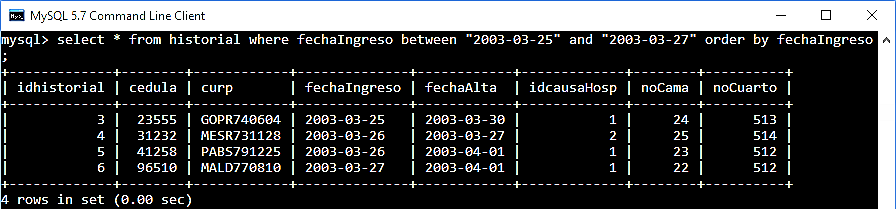
\includegraphics[width=\textwidth]{img/catorce.png}
			\label{fig:catorce}
			\caption{Pacientes que se encuentran en el intervalo indicado}
		\end{center}
	\end{figure}
	Después obtenemos el numero de registros de aquellos pacientes con causa de hospitalización igual a dos.
	%select count(*) from historial where idcausahosp=2;%
	\begin{figure}[H]
		\begin{center}
			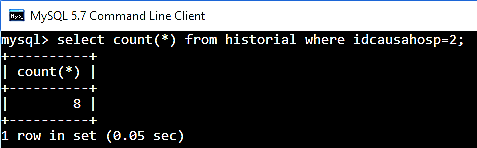
\includegraphics[width=\textwidth]{img/quince.png}
			\label{fig:quince}
			\caption{Numero de pacientes con cierto ID}
		\end{center}
	\end{figure}
	Los siguientes ejercicios involucran modificar el contenido de la base de datos, lo primero fue actualizar el teléfono del medico Omar cortes Landeros.
	\begin{lstlisting}
	select nombre, tel from medico where nombre like "Cort% Lan% Omar%"; -- Buscamos al medico
	update medico set tel=55555577 where nombre like "Cort% Lan% Omar%"; -- Actualizamos
	select nombre, tel from medico where nombre like "Cort% Lan% Omar%"; -- Y observamos los cambios
	\end{lstlisting}
	\begin{figure}[H]
		\begin{center}
			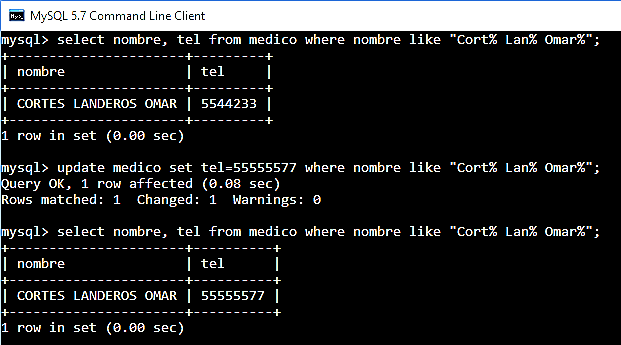
\includegraphics[width=\textwidth]{img/16.png}
			\label{fig:16}
			\caption{Proceso para poder actualizar el teléfono del doctor requerido}
		\end{center}
	\end{figure}
	A continuación se cambió el domicilio de los neurólogos a "Viven en el hospital".
	\begin{lstlisting}
	select nombre, dir from medico where idEsp=(select idEsp from Especialidad where descEsp like "Neur%"); --Observamos a todos los neurologos
	
	update medico set dir="Viven en el hospital" where idEsp=(select idEsp from Especialidad where descEsp like "Neur%"); -- Les modificamos su direccion
	\end{lstlisting}
	\begin{figure}[H]
		\begin{center}
			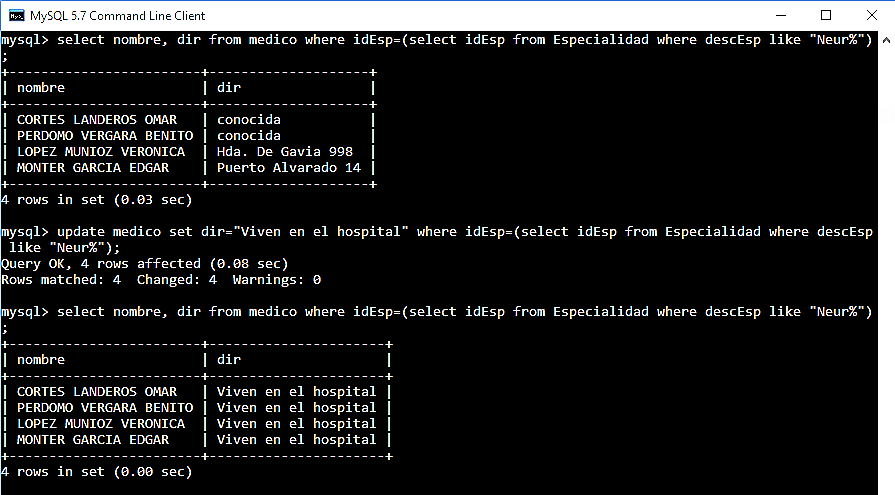
\includegraphics[width=\textwidth]{img/17.png}
			\label{fig:17}
			\caption{Consulta y actualización necesarias para cambiar la dirección de los neurólogos}
		\end{center}
	\end{figure}
	En este ejercicio se dio de alta a dos médicos uno siendo urologo y otro ginecólogo.
	\begin{lstlisting}
	insert into medico values (989898,"Garcia Cebada Miguel", "En su casa", (select idEsp from especialidad where descEsp like "Urolo%"), 55555556), (989899,"Lopez Lopez Kala","En su casa", (select idEsp from especialidad where descEsp like "Ginec%"),55555557); -- Insertamos los nuevos medicos
	
	select * from medico where cedula in(989898,989899); --Visualizamos los campos
	\end{lstlisting}
	\begin{figure}[H]
		\begin{center}
			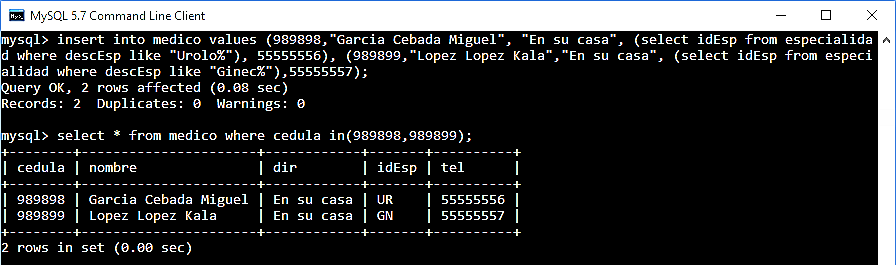
\includegraphics[width=\textwidth]{img/18.png}
			\caption{Insertamos dos nuevos médicos y comprobamos su existencia}
			\label{fig:18}
		\end{center}
	\end{figure}
	Luego, para aquellos pacientes que fueron dados de alta en diciembre de 2009, se cambió su dirección.. a "DESCONOCIDA....."
	\begin{lstlisting}
	select p.nombre, p.dir, h.fechaAlta	from paciente p, historial h where h.curp=p.curp and h.fechaAlta between "2009-12-01" and "2009-12-31" order by 3; -- Vemos los datos de los pacientes que coinciden con la busqueda deseada
	
	update paciente p, historial h set p.dir="DESCONOCIDA......" where h.curp=p.curp and h.fechaAlta between "2009-12-01" and "2009-12-31"; -- Procedemos a modificar esos pacientes
	
	select p.nombre, p.dir, h.fechaAlta	from paciente p, historial h where h.curp=p.curp and h.fechaAlta between "2009-12-01" and "2009-12-31" order by 3; -- Visualizamos los cambios
	\end{lstlisting}
	\begin{figure}[H]
		\begin{center}
			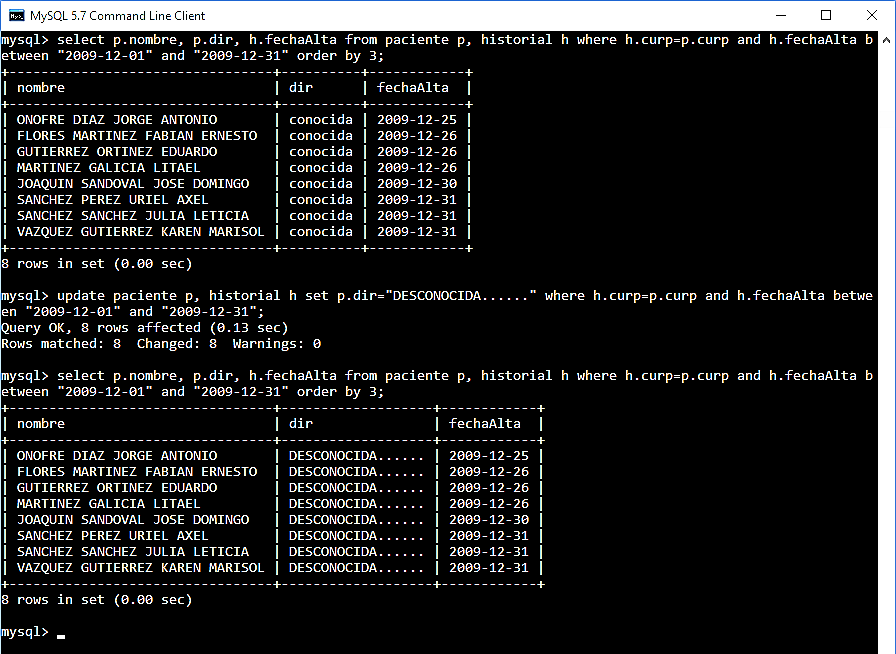
\includegraphics[width=\textwidth]{img/19.png}
			\label{fig:19}
			\caption{A los pacientes que fueron dados de alta en 2009 les cambiamos su dirección con este conjunto de instrucciones}
		\end{center}
	\end{figure}
	Finalmente eliminamos los pacientes que fueron atendidos por el medico Samuel Duran Becerril
	\begin{lstlisting}
	delete from paciente p, medico m, historial h where p.curp=h.curp and h.cedula=m.cedula and m.nombre like "Dura% Bece% Samu%";
	
	select p.curp, p.nombre, m.nombre from paciente p, medico m, historial h where p.curp=h.curp and h.cedula=m.cedula and m.nombre like "Dura% Bece% Samu%";
	
	delete from paciente where curp in("BBJG881021","MCGI910122","VELF890818");
	
	alter table historial drop foreign key FK_historial_2;
	
	alter table historial add foreign key(curp) references paciente(curp) on delete cascade on update cascade;
	\end{lstlisting}

	\section{Conclusiones}
	En un inicio los ejercicios de esta práctica fueron sencillos para poco a poco aumentar su complejidad y mezclar bastantes cosas vistas a lo largo de las prácticas anteriores lo que finalmente permite reforzar estos conocimientos mediante su uso con nuevos temas como lo son en este caso de altas, bajas y cambios.
	\bibliography{bibliografia} 
	\bibliographystyle{ieeetr}
\end{document}